\providecommand{\main}{..}
\documentclass[main.tex]{subfiles}

\begin{document}
\chapter{Software Design}

\section{System Design Overview}
\subsection{Microprocessor Platform}
The streaming capabilities and digital signal processing requirements of the system necessitated the choice of an appropriate microprocessor platform. 
A purely embedded solution was initially considered due to the availability of networking stacks such as FreeRTOS+UDP/IP and Light Weight IP (LWIP), the latter of which is available for ARM mbed platforms. This however would have limited audio and networking related software options that are available for general purpose operating systems such as Linux or QNX.

\medskip
As this was the first prototype for the project, the decision was made to select a Linux based platform as this would allow flexibility in the use of audio and streaming tools that are available for the OS. Benchmarking was conducted for potential platforms that would meet the system performance requirements as outlined in chapter 1, they are outlined in table \ref{table:HWPlatforms}.

\begin{table}[H]
    \centering  
    \caption{Benchmarking of Microprocessor Platform Specifications}
    \begin{tabu} to 0.8\textwidth { | l | l | l | l | l | l | }
        \hline
        \textbf{PLATFORM} &  \textbf{CPU} & \textbf{RAM} & \textbf{DAC} & \textbf{WLAN} & \textbf{PRICE}  \\
        \hhline{|=|=|=|=|=|=|}
        Raspberry Pi 3B & ARM Cortex-A5 & 1GB & NO & YES & £34.00 \\
        & 1.4GHz quad-core & & & & \\
        \hline
        Hardkernel Odroid-CO & ARM Cortex-A5 & 1GB & NO & NO & £32.97 \\
        & 1.5GHz quad-core & & & & \\
        \hline
        iMX233-OLinuXino-MAXI & ARM 926EJ-S & 64MB & YES & NO & £42.13 \\
        & 454MHz single-core & & & & \\
        \hline
        Blueberry Pi & ARM Cortex-A7 & 64MB & NO & YES & n/a \\
        & 1.2GHz single-core & & & & \\
        \hline
        Raspberry Pi Zero W & ARM 1176JZF-S & 512MB & NO & YES & £9.00 \\
        & 1.0GHz single-core & & & & \\
        \hline
        
        
    \end{tabu}
    
    \label{table:HWPlatforms}
    \end{table}

\medskip
%high performance boards (RPI3 & odroid)
%own board (blueberry pi & IMX6)

\medskip
With a single core Broadcom BCM2835 1GHz CPU, 500MB of RAM and no option to implement an eMMC over an SD card, the Raspberry Pi Zero W is significantly under-powered when compared to the other platforms. 
However, the much reduced cost of the device at approximately £9.00\cite{RpiPrice} is significantly less expensive than its counterparts. The very small size of the board, 65x30mm, was also desirable as it would take up much less space on the master PCB housed within the rear enclosure of the cabinet. 
The wiringPi library is also compatible with the Raspberry Pi Zero W (RPZW) which would be convenient when interfacing with hardware peripherals such as the DAC, power-amplifier and user controls. The inclusion of a built in WLAN transceiver is particularly advantageous as this removes the need for a separate WLAN module/IC. 

\medskip
After careful consideration, this platform was selected due to the reasons outlined above. 
The chosen Linux distribution was Debian as it is the standard OS for the raspberry pi and allows easier configuration for real-time audio than other popular distributions such as Ubuntu. 
After the project was completed, further testing was carried out using the Odroid C0 in an attempt to gauge how the increased performance of the platform over the Raspberry Pi affected the performance of the overall system. 

\subsection{Audio Streaming Platform}
Several streaming platforms and tools were benchmarked with regards to requirements as outlined in chapter 1. 
With many options under Linux, two potential approaches to implementing streaming were derived. 
A raw streaming protocol could be implemented at a low level or, a sound server with necessary streaming capabilities and a suitable C++ API could be used in order to distribute multiple streams to different speakers.

\medskip
%RTAUDIO & oRTP & raw-sockets

\medskip
%PulseAudio & JACK

\subsubsection{Multicast Audio Streaming Toolkit (MAST)}

\subsubsection{Linphone: Media Streamer 2}

\subsubsection{PulseAudio Audio Server}

\subsubsection{oRTP}

\subsubsection{JACK/netJACK Audio Server}

\subsection{System Architecture}
\begin{figure}[H]
    \centering
    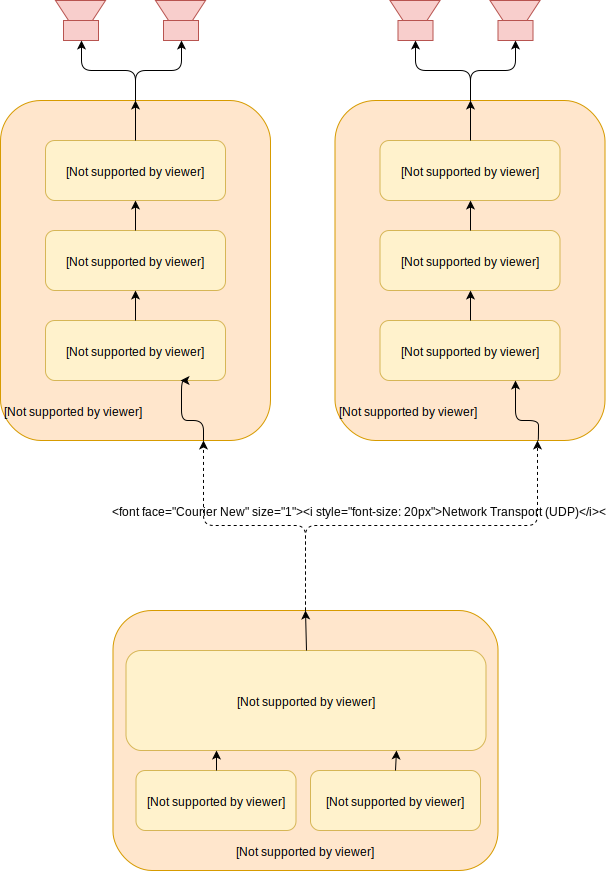
\includegraphics[scale=0.4]{./figs/JACKclients.pdf}
    
    \caption{High-level JACK-based system diagram}
    \label{fig:JACKclients}
\end{figure}

\section{System Startup/Shutdown}

\section{WifiHifi Client}
\subsection{Overview}
%threads, class hierarchy etc
\subsection{Signal Processing}
\subsubsection{Crossover Filters}
\subsubsection{Frequency Correction}
\subsubsection{3-Band EQ}
\subsubsection{Results}
\subsection{ALSA Interface}
% interleaving etc
\subsection{User I/O}

\section{Drift Correction}
\subsection{Overview}
%describe algorithm/maths
\subsection{Implementation}
\subsection{Results}

\section{Desktop Application}
\subsection{Overview}
\subsection{Tone Controls}
\subsection{Connection Protocol}

\end{document}